\chapter{Introduction}

Psychological resilience is generally regarded as positive adaptation to past and ongoing exposure to potential negative effects of stressors. Accordingly, adaptation to stressful or adverse situation is a dynamic process with predictors that can differ between population groups. Within the discipline of developmental psychology, Tuescher and colleagues have provided prospective studies investigating the concept of resilience and its complex underlying mechanisms. As part of a doctoral dissertation, their studies aimed to validate the following research questions:

\begin{itemize}
    \item Does resilience have a positive effect on the willingness to participate in politics, specifically in election?
    \item Does the confrontation with positive or negative statements on politics for people with lower resilience have stronger effects on the willingness to participate in politics?
\end{itemize}

The research group did its poll by selecting people from Mainz, while trying to generalize to the entire German population. The survey data (GBS, n=587) tends to over-represent groups of higher income and higher education, since participants are primarily selected from an academic environment.

Therefore, the validity of assertions about the population beyond the original observation range is affected, even if statements are made conditional upon the available data. The basic premise for standard statistical conclusions, that the training and test set are drawn independently and identically (i.i.d.) from the same probability distribution, does not hold any more. Data sets are rarely generated under ideal conditions with bias pervasive in almost all empirical studies.

To get a complete picture of the subject, the research group consulted the department Data Archives for the Social Sciences. Their data archive service (GESIS) holds representative data of comparable studies in politics and psychology. The acquired sample (GESIS, n=4000) encompasses the German speaking population with permanent residence in Germany. 

This thesis is a practical application to reduce the sampling bias by selecting a maximal representative subsample (MRS) of GBS survey respondents with reference probability distributions from GESIS. The effects of positive and negative treatments on political participation are then analysed in the resulting MRS and compared to the initial GBS data [Fig. 1.1].

To evaluate the research questions to a certain required level of significance, it is inevitable to keep the exclusion of instances at a minimum. Pruning the GBS data in any way, narrows the data variance and thus the reach of subsequent studies. This is especially harmful since the initial GBS survey data is already small.

\vspace{20pt}
\begin{figure}[ht]
	\begin{center}
		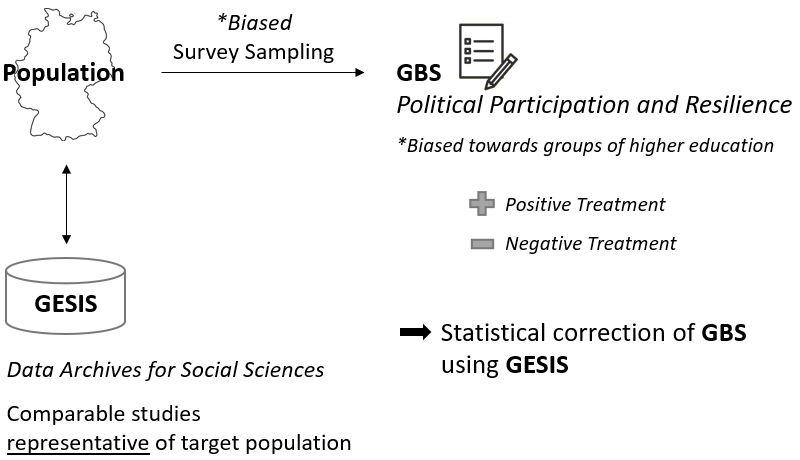
\includegraphics[scale=0.60,angle=0]{fig/overview}
		\label{project}
		\caption{Auxiliary information GESIS linked to GBS so that expected bias can be detected and corrected for. In addition, GBS contains an attribute for positive or negative treatment of survey participants for further analysis.}
	\end{center}
\end{figure}

Depending on the definition of MRS, there are two possible ways to tackle this problem:

\begin{enumerate}

\item Search algorithm with objective scoring function.

\item Try to avoid giving the synthesized data properties that makes it possible for a learning algorithm to distinguish synthesized from non-synthesized example such as if all the synthesized data comes from one of 20 car designs, or all the synthesized audio comes from only 1 hour of car noise. This advice can be hard to follow. 

\end{enumerate}


\section{Related Work}

Incorporate complex survey data features

%It is usually difficult to draw a simple random sample from the population, due to cost and practical considerations such as no comprehensive sampling frame available. As discussed in Sample Design, complex samples, such as surveys involving stratified / cluster sample design, are commonly used in surveys. In a simple random sample, one can assume that observations are independent from %each other. However, in a complex sample design, such as multi-stage samples of schools, classes and students, students from one classroom are likely to be more correlated than those from another classroom. Therefore, as described in Sample Design, in the analysis phase, we need to compensate for complex survey designs with features including, but not limited to, unequal likelihoods of %selection, differences in response rates across key subgroups, and deviations from distributions on critical variables found in the target population from external sources, such as a national Census, most commonly through the development of survey weights for statistical adjustment. If complex sample designs are implemented in data collection but the analysis assumes simple random sampling, %the variances of the survey estimates can be underestimated and the confidence interval and test statistics are likely to be biased (Heeringa, West, & Berglund, 2010). 
%http://ccsg.isr.umich.edu/index.php/chapters/statistical-analysis-chapter#nine

%In a recent meta-analysis of 150 sampled research papers analyzing several surveys with complex sampling designs, it is found that analytic errors caused by ignorance or incorrect use of the complex sample design features were frequent. Such analytic errors define an important component of the larger total survey error framework, produce misleading descriptions of populations and %ultimately yield misleading inferences (Aurelien, West, & Sakshaug, 2016). It is thus of critical importance to incorporate the complex survey design features in statistical analysis. 
%For many of the aforementioned statistical models, various statistical software programs have enabled the analysis of complex survey data features, such as “svy” statement in Stata, and SURVEY procedures in SAS. See Appendix A for more information.  

\section{Outline}

The remainder of this thesis is organized as follows. Section 2 starts with an initial data analysis step and focuses more narrowly on checking assumptions required for model fitting and hypothesis testing, i.e. handling missing values and making transformations of variables. Section 3 discusses the feasibility of learning in a binary classification setting. To estimate model performance in the absence of labeled negatives, standard evaluation metrics are adapted using an initial ranking model. Discriminative ensemble models are trained on positive and unlabaled data in Section 4 to label instances as representative that cannot be distinguished from the out-of-sample distribution. The resulting maximal representative subset of GBS is presented in Section 5 and compared to GBS and GESIS regarding political participation and resilience. Related work is discussed in Section 6 and Section 7 concludes.
